\chapter{动量守恒}

\section{牛顿第三定律}

牛顿第二定律给出了任何物体的加速度与作用在它土面的力之间的关系,在这个基础上,原则上可以解决任何力学问题。例如,为了确定几个粒子的运动,人们可以利用前面一章中所展开的数值方法。但是我们有充分的理由来进一步研究牛顿定律。首先,有一些十分简单的运动不仅可以用数值方法分析,也可以直接进行数学分析。比如:我们知道落体的加速度是$32ft \cdot s^{-1}$后,由这个事实虽然可以用数值方法计算出运动,但是分析这个运动并找到一般解$s=s_0+v_0t+16t^2$,则更为容易也更令人满意。同样,虽然我们可以按数值方法计算简谐振子的位置,但我们也能用分析方法表明一般解是简单的$t$的余弦函数,因此,当存在一种简单而又更为精确的方法以得出结果时,再去用一系列麻烦的算术运算就毫无必要了。同理一个行星由引力决定的绕太阳的运行固然可以用第9章的数值解法逐点地加以计算,从而找到轨道的一般形状,但能够得到准确的形状——分析表明这是一个完整的棚圆——就更好了。

遗憾的是,只有很少问题能够以分析方法精确求解。例如就简谐振子来说,如果弹簧力不是正比于位移,而是更为复杂的话,人们就只得又回到数值解法上来。或者,假如有两个天体绕太阳运行,使天体的总数是三个,那么分析法就无法得出一个简单的运动公式,实际上这个问题只能作数值解。这就是著名的三体问题,它曾经长时间地向人们的分析能力挑战;十分有趣的是,人们花了那么长时间才领悟到也许数学分析的能力是有限的,因而使用数值解法是必要的这个事实。今天,大量无法以分析方法解决的问题已由数值方法解出,那个曾被认为是如此困难的占老的三体问题,已作为常规计算准确地按上一章所描述的方式进行充分的演算后,加以解决了。然而,也有一些两种方法都失效的情况:对简单的问题我们可以用分析方法,对适当困难的问题可以用数值和算术方法;但是对非常困难的问题则这两种方法都不能用了。例如:两辆汽车的碰撞,或者甚至气体中分子的运动,就是一种复杂的问题。在一立方毫米的气体中有数不清的粒子,而试图用这么许多变量(约$10^{17}$个)来作计算将是荒谬的。任何问题,如果不是只有两三个行星绕太阳运行,而是诸如像气体、木块、铁块中的分子或原子的运动,或在球状星团中许多恒星的运动之类这样的问题,我们就不能直接去解,因此只好借助于其他手段。

在那种无法了解细节的情况下,我们需要知道某些一般性质,亦即需要知道作为牛顿定律结果的一般性定理或原则。在第4章讨论过的能量守恒定律就是其中之一。另一个是动量守恒定律,这是本章的课题。进一步研究力学的另一个理由是:有某些运动模式在许多不同的状况下一再重复地出现,因此在一个特定情况下研究这些模式是有益的。例如,我们将研究碰撞,不同类型的碰撞有许多共同之处。又如在流体的流动中,到底是哪一种流体这个问题并没有多大关系,这是因为流动的定律是类似的。我们将研究的其他一些问题是振动及振荡,特别是,机械波的特殊现象——声、杆的振动,等等。

在我们对牛顿定律的讨论中已经解释过:这些定律是一种处理问题的方案,它告诉我们:“要注意力!”而在有关力的性质方面牛顿只向我们讲了两件事。在引力情况中,他留给我们一条完整的力的定律。关于原子间的非常复杂的作用力,他并不知道力的正确的规律;然而,他发现了一条有关力的一般性质的规则,并在第三定律中对此作了阐明,这就是牛顿在有关力的性质上所具有的全部知识——引力定律和\uwave{第三}定律,再没有其他细节了。

牛顿第三定律是:\uwave{作用等于反作用}。

它的含义如下:假设我们有两个小物体,比如说两个粒子,第一个粒子对第二个粒子施加一个力,即用一个一定的力推它。那么,按照牛顿第三定律,第二个粒子同时以大小相等、方向相反的力推第一个粒子;而且,这些力实际上沿同一根线起作用。这就是牛顿提出的假设,或者说定律,它看来是相当准确的,尽管并不严格正确(以后我们将讨论它的误差)。暂时我们将认为作用等于反作用是正确的。当然,假如有第三个粒子,它不与前两个粒子在同一条直线上,则这个定律并不意味着作用在第一个粒子上的总的力等于作用在第二个粒子上的总的力,因为,比方说,第三个粒子对这两个粒子中的每一个都要施加推力。结果作用在前两个粒子上的总效应是在某个别的方面上,从而一般说来,作用在前两个粒子上的力大小既不相等,方向也不相反。然而,作用在每个粒子上的力总可以分解为若干部分,每一个与之相互作用的粒子都有一份贡献或一个部分。因而,每一对粒子都有相应的彼此相互作用的分量,它们大小相等、方向相反。

\section{动量守恒}

现在来看一下,上述联系有什么有趣的结果?为了简单起见,我们假设只有两个互相作用的粒子,质量可能不同,并分别编为1号及2号。它们之间的力相等而方向相反;这会有什么结果呢?按照牛顿第二定律,力是动量对时间的变化率,于是我们得出粒子1的动量$p_1$的变化率等于粒子2的动量$p_2$变化率的负值,即
\begin{equation}
    \label{Eq:I:10:1}
    \frac{dp_1}{dt}=-\frac{dp_2}{dt}
\end{equation}
现在,如果变化率总是数值相等、方向相反,就可知道粒子1动量的总变化与粒子2动量的总变化数值相等、方向相反;这意味着,如果我们把粒子1的动量与粒子2的动量相加,那么由于粒子之间相互作用力(称为内力)引起的两个粒子动量之和的变化率为零,即
\begin{equation}
    \label{Eq:I:10:2}
    \frac{d(p_1+p_2)}{dt}=0
\end{equation}
在这个问题中假定没有其他作用力。如果这个和的变化率总是零,这正是量$(p_1+p_2)$不发生变化的另一种说法(这个量也可写成$m_1v_1+m_2v_2$,并称为这两个粒子的总动量)。现在我们得出两个粒子的总动量不因它们之间的任何相互作用而改变的结论。这个说法表示了在这个特例下的动量守恒定律。我们断言:如果两个粒子间存在着任何类型的力(不管这个力怎样复杂),我们在力作用之前及力作用之后去测量或计算$(m_1v_1+m_2v_2)$,即两个动量之和,则结果总是相等的,也就是说,总动量是一个常数。

假如我们把论证引申到更复杂的三个或多个相互作用粒子的情况,那么很明显,当只考虑内力时,所有粒子的总动量保持不变,因为其中一个粒子由另一个粒子引起的动量的增加,恰好严格地被前者引起的后者动量的减少所补偿。也就是说,所有的内力将互相抵消,因此不可能改变粒子的总动量。于是,如果没有来自外界的力(外力),那么就没有什么力可以改变总动量,因此总动量是一个常数。

值得一提的是,如果存在一些并非来自所说的粒子间的相互作用的力:假定我们把相互作用的粒子隔离开来,这时会出现什么情况?如果只有相互作用力,那么同以前一样,无论这些力多么复杂,粒子的总动量不变。反之,假定还有来自隔离开来的那一群以外的粒子的作用力。我们称任何外部物体施加于内部物体的力为外力。以后我们将证明所有外力之和等于所有内部粒子动量总和的变化率。这是一个非常有用的定理。

如果没有净的外力,一群相互作用粒子的总动量守恒可以表示为
\begin{equation}
    \label{Eq:I:10:3}
    m_1v_1+m_2v_2+m_3v_3+...=\text{常数}
\end{equation}
这里将粒子的质量和相应的速度顺序编为1,2,3,4,…等。对每个粒子,牛顿第二定律的一般表述是
\begin{equation}
    \label{Eq:I:10:4}
    f=\frac{d}{dt}(mv)
\end{equation}
特别是对力和动量在任何给定方向上的分量也同样成立;这样作用在一个粒子上的力的$x$
分量就等于该粒子动量变化率的$x$分量,即
\begin{equation}
    \label{Eq:I:10:5}
    f_x=\frac{d}{dt}(mv_x)
\end{equation}
对$y$和$z$方向也如此。所以方程式(\ref{Eq:I:10:3})实际上是三个方程,每个方向一个。

除动量守恒定律外,牛顿第二定律还有另一个有趣的结果,现在先提一下,以后再证明。这个原理就是:无论我们保持静止状态,还是沿一条直线作匀速运动,物理定律将都是相同的。例如,一个在飞机上拍皮球的孩子,会发现皮球跳得和他过去在地面上拍时一样高。即使飞机以极高速度飞行,只要它不改变飞行速度,物理定律在孩子看来总是和飞机静止时完全一样。这称为相对性原理。当我们在这里使用这个原理时,将称它为“伽利略相对性”,以与爱因斯坦所作的更仔细的分析相区别,后者我们将在以后研究。

我们刚从牛顿定律推导出了动量守恒定律,由此出发,我们可以接下去找出一些描写碰撞的定律。但是为多样化起见,同时也为了阐明一种在物理学上可用于其他情况(比方说,人们也许并不知道牛顿定律,也许另辟途径)的推理方式,我们将从一个完全不同的观点讨论碰撞定律。我们的讨论将从上述伽利略相对性原理出发,而以得出动量守恒定律告终。

我们将从下列假定出发:我们以一定速度运动并观察自然界时,自然界在我们看来和我们静止不动时完全相同。在讨论那种两个物体碰撞后粘在一起,或者来到一起再弹开的情况之前,我们将首先考虑用弹簧或其他东西联结在一起的两个物体,突然放开它们,使它们受到弹簧或者某种轻微爆炸所造成的推力的情形。而且,我们将只考虑一个方向上的运动。我们先假定,两个物体完全相同、十分对称,接着两者之间发生了轻微爆炸。爆炸后,其中一个物体将以速度$v$向右运动,另一个物体将以速度v向左运动。由于这两个物体是全同的,因而没有什么理由认为它们对左或右会有所偏爱,故两个物体的行为应该是对称的。因此,认定另一物体以速度$v$向左运动看来是合理的。这里阐明了一种在许多问题中都十分有用的思维方式,如果我们只从公式入手,那就显不出来了。

我们这个实验的第一个结论是相同的物体将有相等的速率,现在假设两个物体由不同材料比如说铜和铝制成,并令它们的质量相等。我们将假定,如果用两个质量相等的物体做实验,即使它们不是全同的,它们的速度也将是相等的。有人可能反驳说:“但是你知道,你可以反过来,不必去作假设。你可以定义在这个实验中获得相等速度的两个物体的质量为相等的质量。”我们按照这个建议,并在铜块与体积很大的铝块之间作一次轻微爆炸,铝块是如此之重,以至于铜块飞出去后,铝块几乎不动。由于铝太多,因而我们把铝块减少到只剩下很薄一片,于是当我们再作一次爆炸时,铝块飞走了,而铜块却几乎不动。这说明铝又太少了。很明显,在两种铝的数量之间有某个正确的数值;于是我们继续调整铝的数量直至速度相等为止。好,现在我们反过来,并认为当速度相等时,质量也相等。这似乎只是一个定义,看来很奇怪,我们居然可以把一些物理定律变成仅仅是一些定义。然而,这里已经包含了某些物理定律,假如我们采纳这个质量相等的定义,我们立即就可得到如下的一条定律。

假设我们从上面的实验知道,两块材料A与B(铜和铝)具有相等的质量。我们用上述的同样方式将铜块和第三块材料,比如金块,进行比较,并确认它的质量等于铜块的质量。如果我们现在用铝和金做实验,在逻辑上并不能说明这些质量必须相等;然而实验表明它们实际上是相等的。所以通过实验,我们发现了一条新的定律。这条定律的一种说法可能是这样的:如果两个物质的质量分别等于第三个物质的质量(由在这个实验中速度相等来确定),那么它们彼此相等(这个表述完全不能从用于有关数学量的假设的相似的陈述中推得)。从这个例子我们可以看到,假如我们不小心的话,我们会多么轻易地推出结论!说速度相等时质量相等,这绝不仅仅是一个定义,因为说质量相等就含有数学上有关相等的定律的意思,而这个相等的定律又可反过来对有关实验作出预言。

作为第二个例子,假设实验时用某一强度的爆炸使A、B两个物体获得一定的速度,从而发现它们相等;那么如果我们再使用更强烈的爆炸,这时所获得的速度是不是还相等呢?同样在逻辑上根本不能确定这个问题,但实验证明确实如此。这样,我们又有了一条定律,它可以表述为:如果在某一速度时按照速度相等方法来测定两个物体具有相等质量,则在另一个速度下测量,它们也将有相同的质量。从这些例子中我们看出,表面上看来只是一个定义的东西实际上包含了某些物理定律。

在下面的论证中,我们将假设:当在两个物体间发生爆炸时,相等的质量将具有数值相等、方向相反的速度这个命题成立。在相反的情况下,我们将作另一个假设:如果两个以相等的速度在相反的方向上运动的全同物体碰撞后被某种粘胶粘在一起,那么碰撞后它们将以什么方式运动呢?这又是一个对左和右没有特别偏重的对称的情况,所以我们假定它们将保持静止。我们还要假定,任何两个质量相同的物体,即使由不同材料制成,当它们以相等的速度沿相反的方向运动而发生碰撞并粘在一起时,它们碰撞后将保持静止。

\section{动量是守恒的}
我们可以用实验来验证上述假设:即,第一,如果两个相等质量的静止物体发生爆炸后分开时,它们将以同样的速率分开运动;第二,两个相等质量的物体以同样的速率相向运动,碰撞并粘合后,它们将停止运动。我们可以利用一个称为气垫的惊人的发明来做实验,它能摆脱不断使伽利略深感麻烦的摩擦力(图\ref{figure:直线气垫端视图})。伽利略不能用光滑的东西来做实验,因为那些物体不能自由地滑动,但是在今天,加上一个神奇的凹槽\footnote{原文为touch(接触),疑为trough(槽)之误(air trough即气垫)。——译者注}后,我们就能摆脱掉摩擦力。我们的物体正如伽利略所宣称的那样,可以毫无困难地以不变的速度滑动。这是通过以空气来托起物体而实现的。因为空气只有极其微小的摩擦力,当不加力时,物体实际上就以不变的速度滑行。首先,我们使用两个经过精心制作具有同样的重量或质量的滑块(实际上是测出了它们的重量,但是我们知道重量是正比于质量的),在两个滑块间的一个封闭气缸中放进一个小的雷管(图\ref{figure:带有爆破作用气缸附件的滑块截面图})。开始时,将两个滑块静止置放在槽的中心,然后利用电火花引爆雷管,迫使它们分开。这时会出现什么呢?如果在它们飞开时速率相等,就应当同时到达气垫的两端。到达两端后,它们实际上又将以相反的速度弹回,然后又跑到一起,并停在开始运动时的起点——中心处。这是一个很好的试验;经过实践以后,结果正如上所述(图\ref{figure:两个质量相等的物体的作用-反作用实验的示意图})。
\begin{figure}[htbp]
    \centering
    \begin{minipage}[t]{0.4\textwidth}
        \centering
        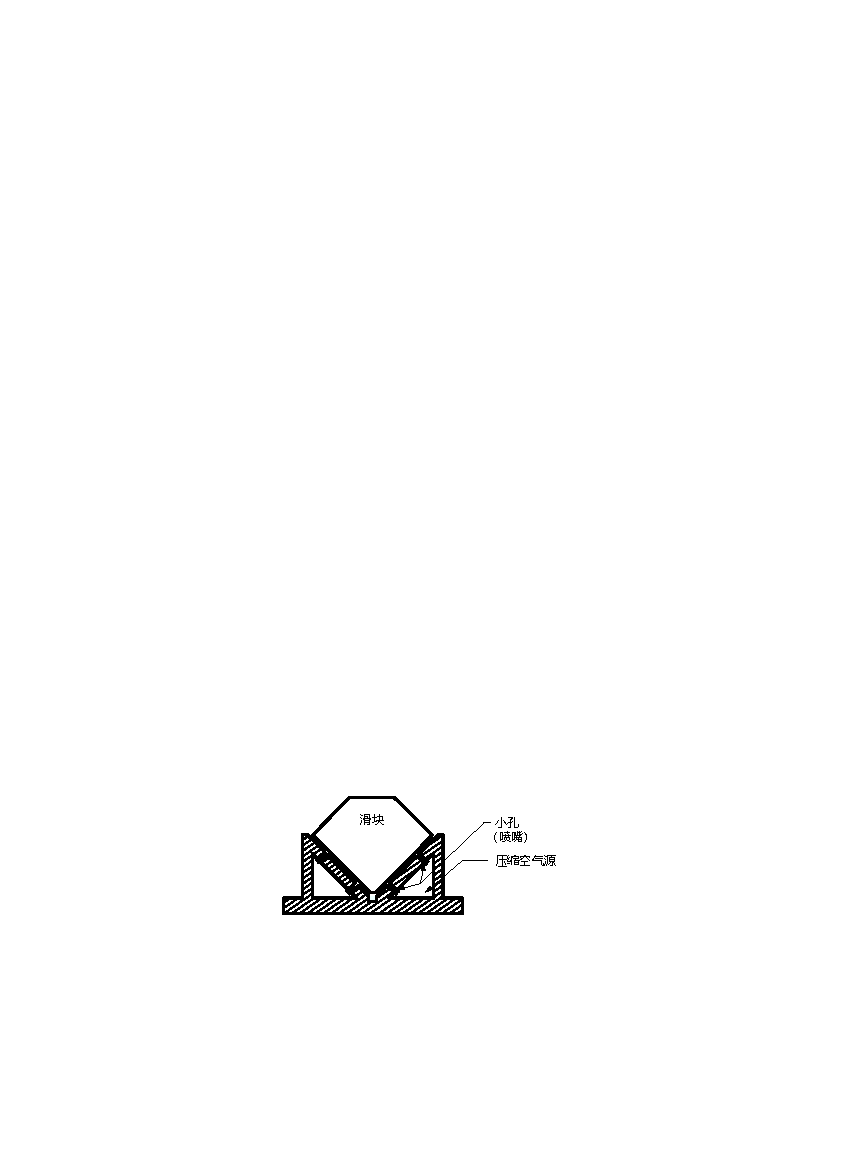
\includegraphics[width=5cm]{Chapter10/直线气垫端视图}
        \caption{直线气垫端视图}
        \label{figure:直线气垫端视图}
    \end{minipage}
    \begin{minipage}[t]{0.4\textwidth}
        \centering
        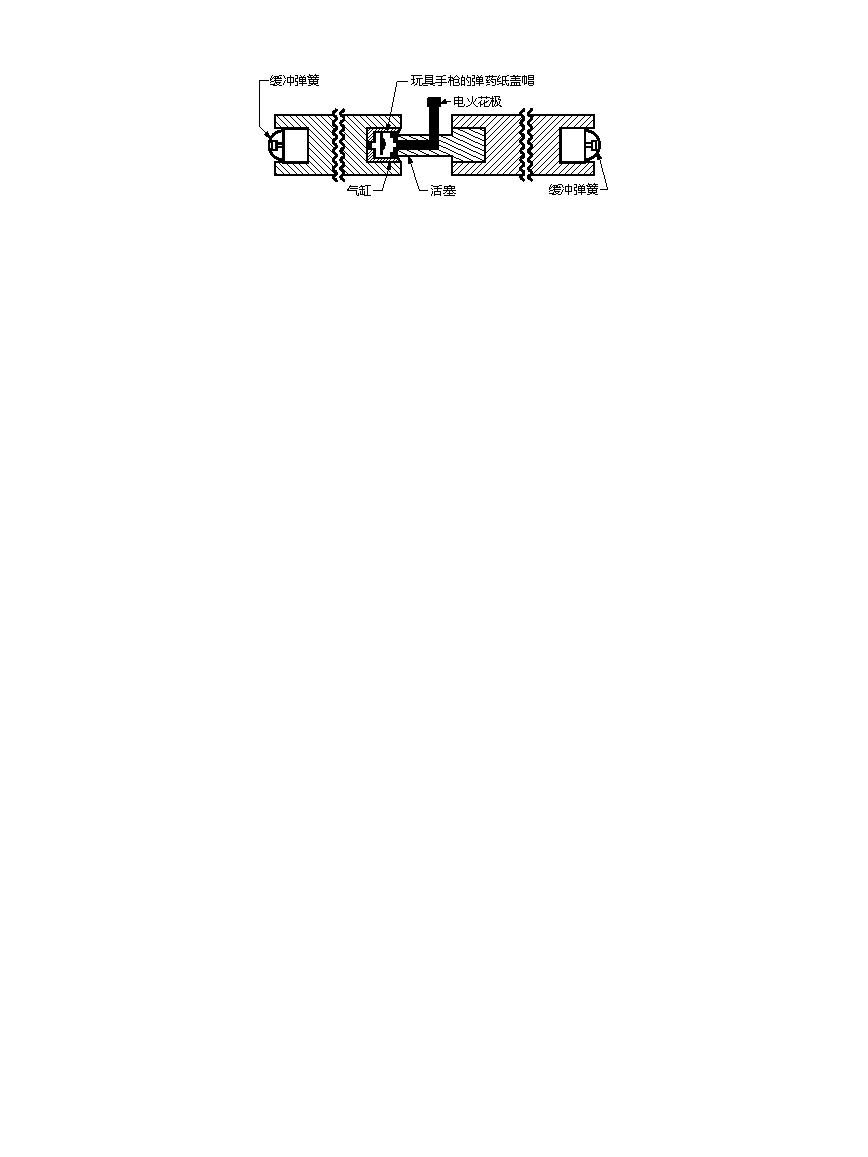
\includegraphics[width=5cm]{Chapter10/带有爆破作用气缸附件的滑块截面图}    
        \caption{带有爆破作用气缸附件的滑块截面图}
        \label{figure:带有爆破作用气缸附件的滑块截面图}
    \end{minipage}
\end{figure}

\begin{figure}[htbp]
    \centering
    \begin{minipage}[t]{0.4\textwidth}
        \centering
        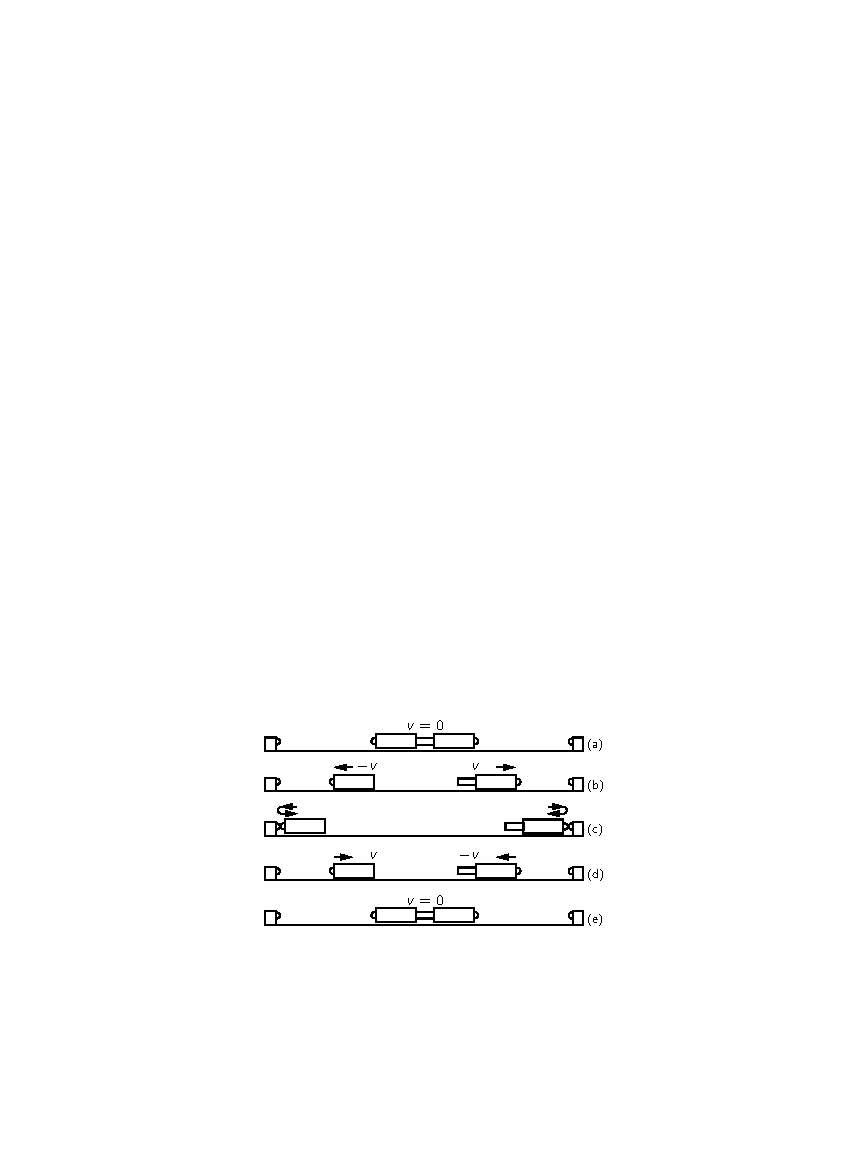
\includegraphics[width=5cm]{Chapter10/两个质量相等的物体的作用-反作用实验的示意图}
        \caption{两个质量相等的物体的作用-反作用实验的示意图}
        \label{figure:两个质量相等的物体的作用-反作用实验的示意图}
    \end{minipage}
    \begin{minipage}[t]{0.4\textwidth}
        \centering
        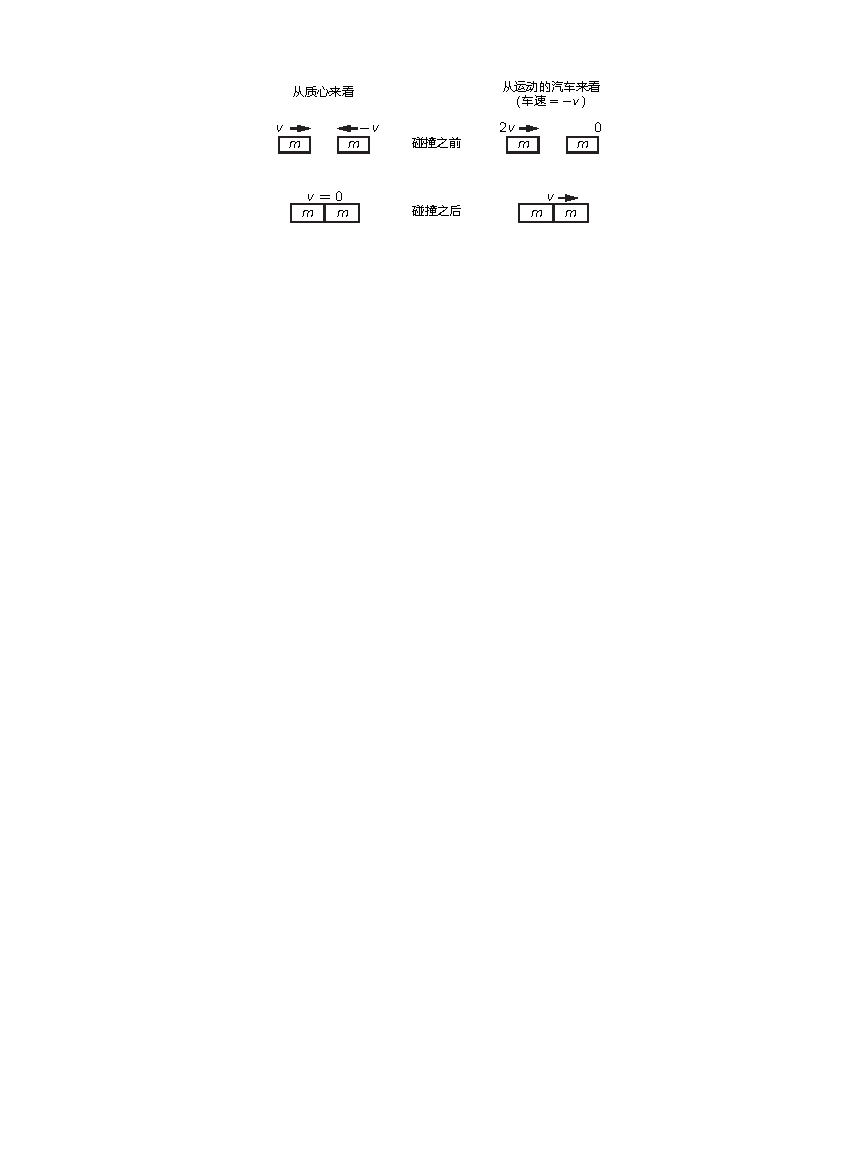
\includegraphics[width=5cm]{Chapter10/质量相等的物体进行的非弹性碰撞的两种看法}    
        \caption{质量相等的物体进行的非弹性碰撞的两种看法}
        \label{figure:质量相等的物体进行的非弹性碰撞的两种看法}
    \end{minipage}
\end{figure}

接下来,我们要解决的是在稍微复杂一些的情况下会发生什么。假设我们有两个质量相等的物体,一个以速度$v$运动,另一个静止不动,它们碰撞后结合在一起;那时又将发生什么情况?结果是一个质量为$2m$的物体以一个未知速度移动。速度多大呢?问题就在于此。为了找到答案,假定当我们驱车前进时,物理规律在我们看来和静止时完全一样。我们从两个质量相等以相同的速率$v$沿相反的方向运动的物体发生碰撞后,将静止不动出发。现在假设在发生这种情况时,我们乘在一辆以速度一$v$开行的汽车上。那么它看上去像什么呢?由于我们随着两个相向运动的物体中的一个一起前进,因而这一个物体在我们看来速度为0。而另一个以速度$v$向相反方向运动的物体,在我们看来就以速度$2v$向我们走来(图\ref{figure:质量相等的物体进行的非弹性碰撞的两种看法})。最后,在碰撞后结合起来的物体看来以速度$v$经过。因此我们得出结论,一个速度为$2v$的物体碰到另一个静止的质量相等的物体时,结果将以速度$v$运动,或者用数学上完全等价的方式来说是:一个速度为$v$的物体撞在另一个
\begin{wrapfigure}{r}{0.4\textwidth}
    \centering
    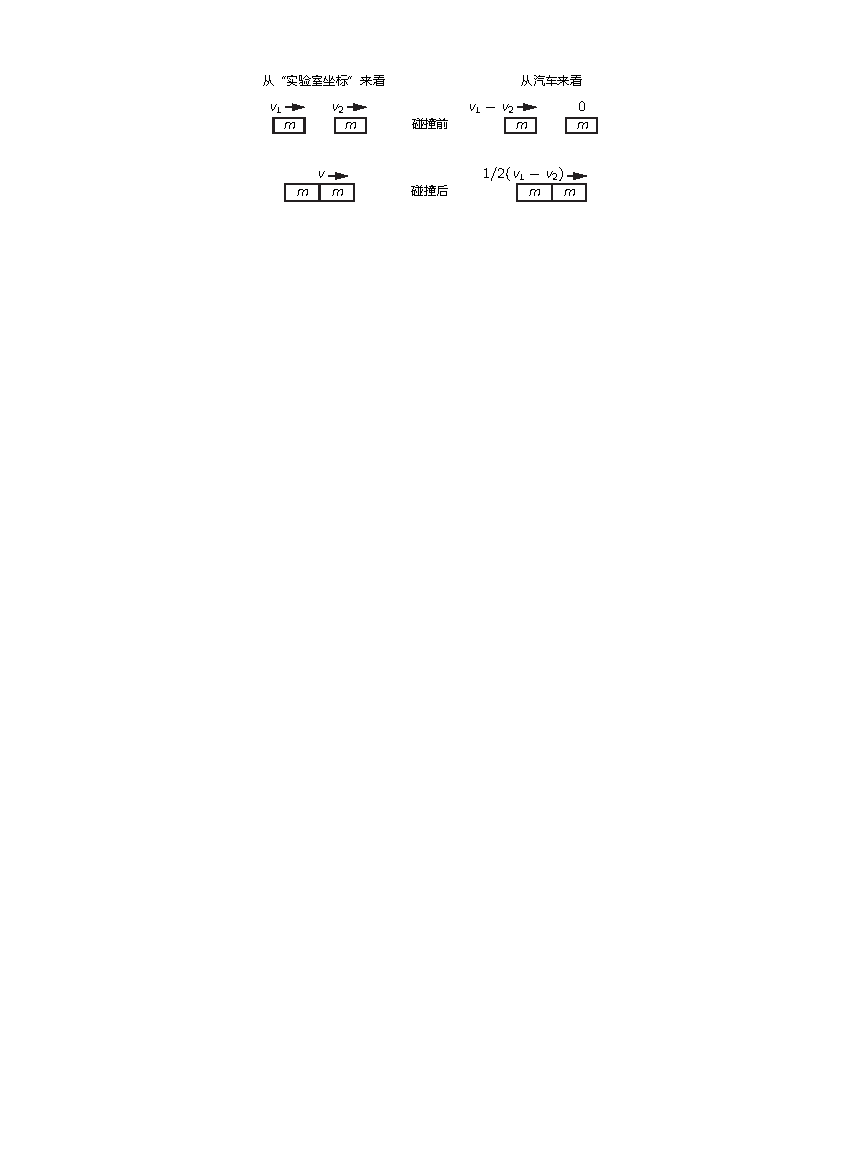
\includegraphics[width=0.35\textwidth]{Chapter10/质量相等的物体进行的另一种非弹性碰撞的两种看法}
    \caption{质量相等的物体进行的另一种非弹性碰撞的两种看法}
    \label{figure:质量相等的物体进行的另一种非弹性碰撞的两种看法}
\end{wrapfigure}
静止物体上并结合在一起时,将产生一个以速度$v/2$运动的物体。注意,如果我们将事前的质量与速度分别相乘再相加得到$mv+0$,与我们将事后的每一个物体的质量与速度相乘,即$2m$乘以$v/2$所得的答案相同。这就告诉我们一个速度为$v$的物体撞在一个静止的物体上时会出现什么情况。

我们可以用完全同样的方式推导出当两个质量相等的物体以任意两种速度相碰撞时会出现什么情况。

假设我们有两个质量相等的物体,分别具有速度$v_1$及$v_2$,它们碰撞并结合在一起。试问碰撞后,它们的速度是多少?我们再乘上一辆速度为$v_2$的汽车来看,则一个物体就像是静止的,而另一个物体就像具有$(v_1-v_2)$的速度,于是我们就得到了同以前一样的情况。当所有这一切都完成后,它们相对于汽车将以$(v_1-v_2)/2$的速度运动。那么它们相对于地面的实际速度是多少呢?答案是$v=(v_1-v_2)/2+v_2=(v_1+v_2)/2$(图\ref{figure:质量相等的物体进行的另一种非弹性碰撞的两种看法})。我们再次注意到
\begin{equation}
    \label{Eq:I:10:6}
    mv_1+mv_2=2m \cdot \frac{(v_1+v_2)}{2}
\end{equation}

于是利用这个原理,对于任何质量相等的物体碰撞后结合在一起的情况,我们都能加以分析。事实上,我们虽然只是计算了一维的情况,但是假如我们坐在一辆沿某个倾斜方向运动的汽车上,我们就可以对更为复杂的碰撞找出更多的东西。这里原理是相同的,只是细节上更加复杂而已。

为了从实验上检验一个以速度$v$运动的物体与另一个速度为0的质量相等的物体碰撞在一起后,是否会组成一个以速度$v/2$运动的物体,我们可以用气垫装置进行如下的实
\begin{wrapfigure}{l}{0.4\textwidth}
    \centering
    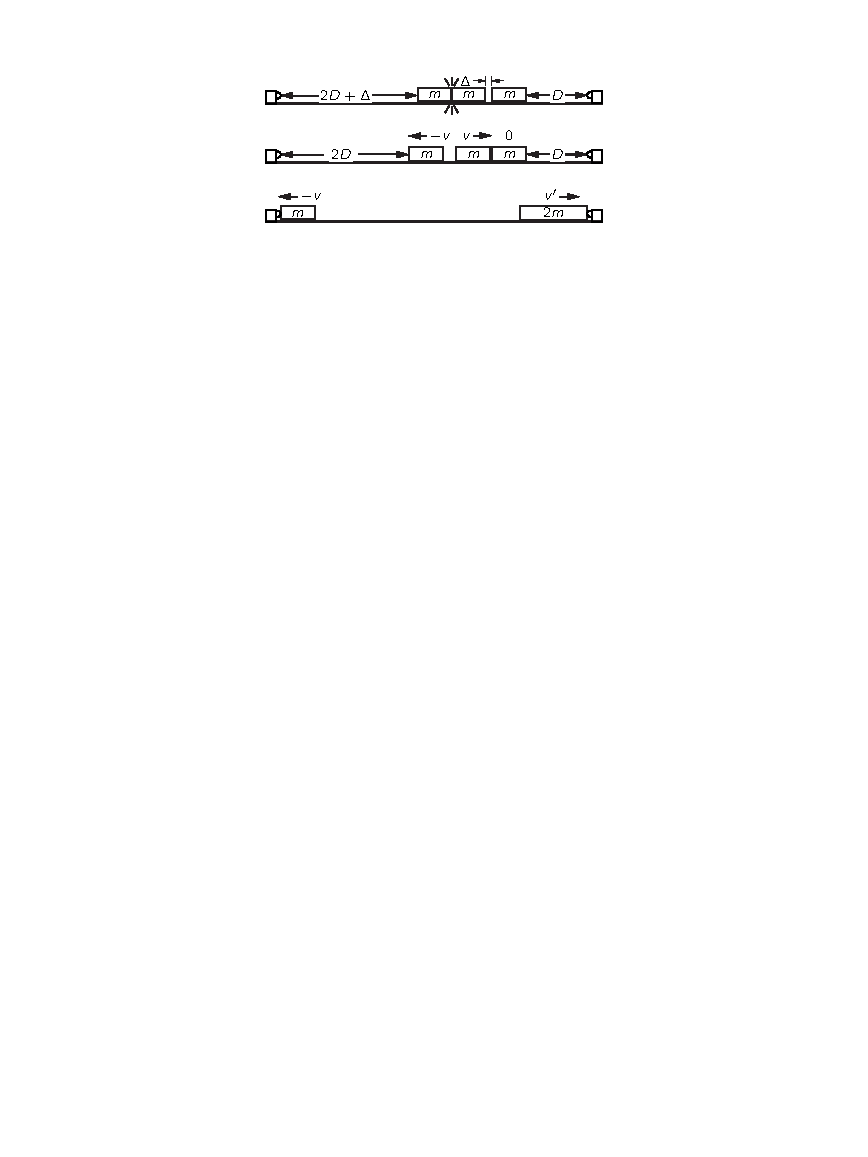
\includegraphics[width=0.35\textwidth]{Chapter10/验证以速度v运动的质量为m的物体与一个质量相同的静止物体}
    \caption{验证以速度$v$运动的质量为$m$的物体与一个质量相同的静止物体碰撞后结合在一起以质量$2m$、速度$m/2$运动的实验}
    \label{figure:验证以速度v运动的质量为m的物体与一个质量相同的静止物体}
\end{wrapfigure}
验。在气垫中放入三个质量相等的物体,其中两个物体开始时由爆破汽缸装置连接在一起,第三个物体非常靠近,但和它们稍微隔开一点点,它还带有一个粘性缓冲器以至于在另一个物体碰上它时,就会和它粘在一起。现在,在爆炸后一刹那,我们有两个质量为$m$,分别以相等而相反的速度$v$运动的物体。过一会儿其中一个物体将碰撞在第三个物体上,构成一个质量为$2m$的物体,我们相信,它将以速度$v/2$运动。我们怎样测出它确实是$v/2$呢?把物体在气垫上的初始位置作这样安排,使得两端的距离不同,而是按 2 : 1 的比例。这样继续以速度$v$运动的第一个物体,在一给定时间内所通过的距离将是那两个连在一起的物体通过的距离的2倍(假定第二个物体在与第三个物体碰撞前只通过一段很小的距离)。质量为$m$的物体与质量为$2m$的物体应当同时到达终点,我们去试一下时,就会发现确实如此(图\ref{figure:验证以速度v运动的质量为m的物体与一个质量相同的静止物体})。

我们要解决的下一个问题是,如果有两个不同质量的物体,情况又会怎样。让我们取一个质量为$m$的物体和一个质量为$2m$的物体,并利用我们的爆炸作用。这时将会发生什么呢?如果爆炸后$m$以速度$v$运动,那么$2m$又以什么速度运动呢?令第二个和第三个质量之间的距离为零,重复我们刚才作过的实验,当我们试一下后,会得出同样的结果,也就是说,起作用的质量$m$和$2m$各达到速度——$v$及$v/2$。这样,$m$与$2m$之间的直接的反作用与先是在$m$和$m$之间对称地反作用,随后$m$又与第三个$m$发生碰撞并结合在一起所得出的结果完全相同。而且,我们还发现,从气垫两端弹回的质量为$m$和$2m$的物体的速度与原来(几乎)完全相反,如果它们粘在一起,就会停止不动。

现在我们要问的另一个问题是:如果具有速度为$v$,质量为$m$的物体与另一个静止的质量为$2m$的物体碰撞并结合在一起,会发生什么情况呢?这个问题利用伽利略相对性原理很容易回答,因为我们只要坐在一辆以速度——$v/2$运动的汽车里观察刚才描写的碰撞就行了(图\ref{figure:m和2m之间的非弹性碰撞的两种看法})。从汽车上看,速度是
\begin{equation*}
v_1^{'}=v-v(\text{汽车})=v+\frac{v}{2}=\frac{3}{2}v \text{ 及 } v_2^{'}=-\frac{v}{2}-v(\text{汽车})=-\frac{v}{2}+\frac{v}{2}=0
\end{equation*}
在碰撞后,质量$3m$在我们看来以速度$v/2$运动。于是我们就得到了碰撞前后的速度比是 3 : 1 的答案:如果一个质量为$m$的物体与一个质量为$2m$的静止的物体相碰撞,并结合在一起,则整个物体就以原先$m$的速度的$1/3$运动。一般的规则又是:各个物体的质量与速度乘积之和保持不变,即$mv+0=3m \times v/3$,这样,我们就一步一步逐渐建立起动量守恒定理。

\begin{figure}[htbp]
    \centering
    \begin{minipage}[t]{0.4\textwidth}
        \centering
        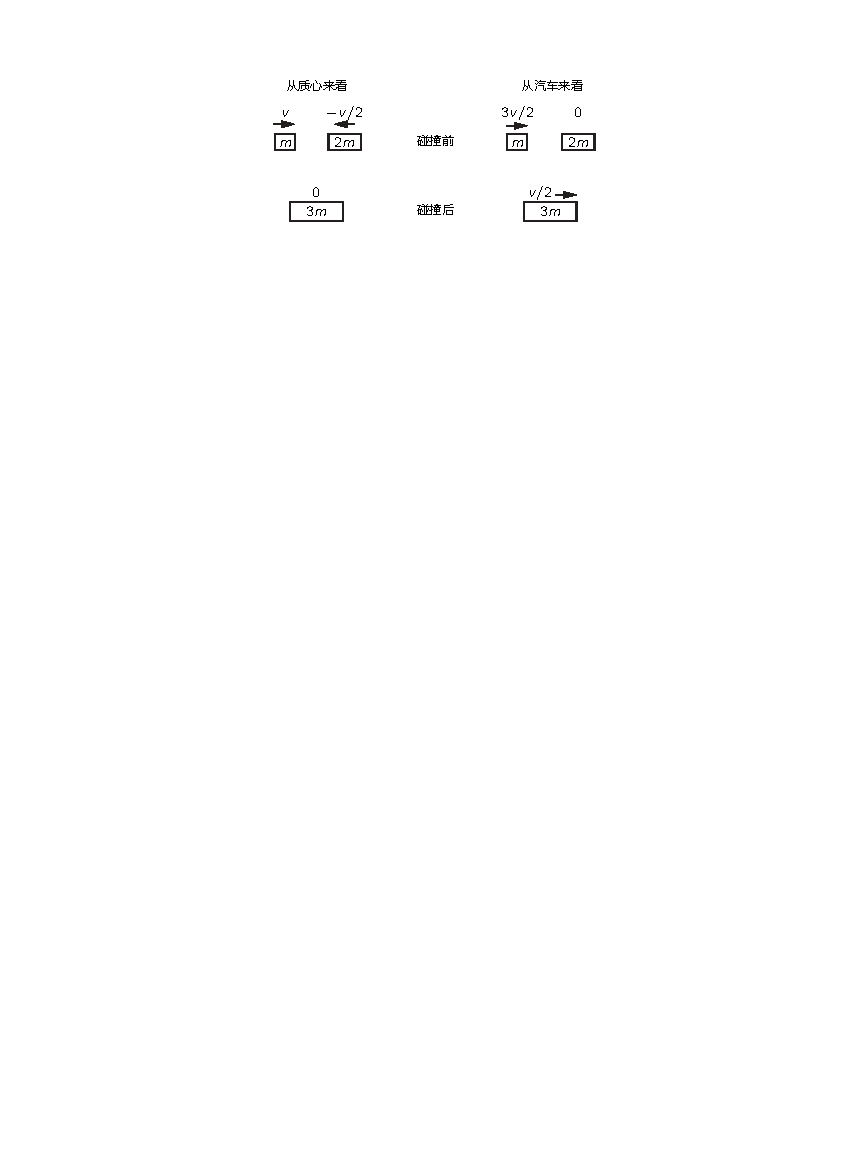
\includegraphics[width=5cm]{Chapter10/m和2m之间的非弹性碰撞的两种看法}
        \caption{$m$和$2m$之间的非弹性碰撞的两种看法}
        \label{figure:m和2m之间的非弹性碰撞的两种看法}
    \end{minipage}
    \begin{minipage}[t]{0.4\textwidth}
        \centering
        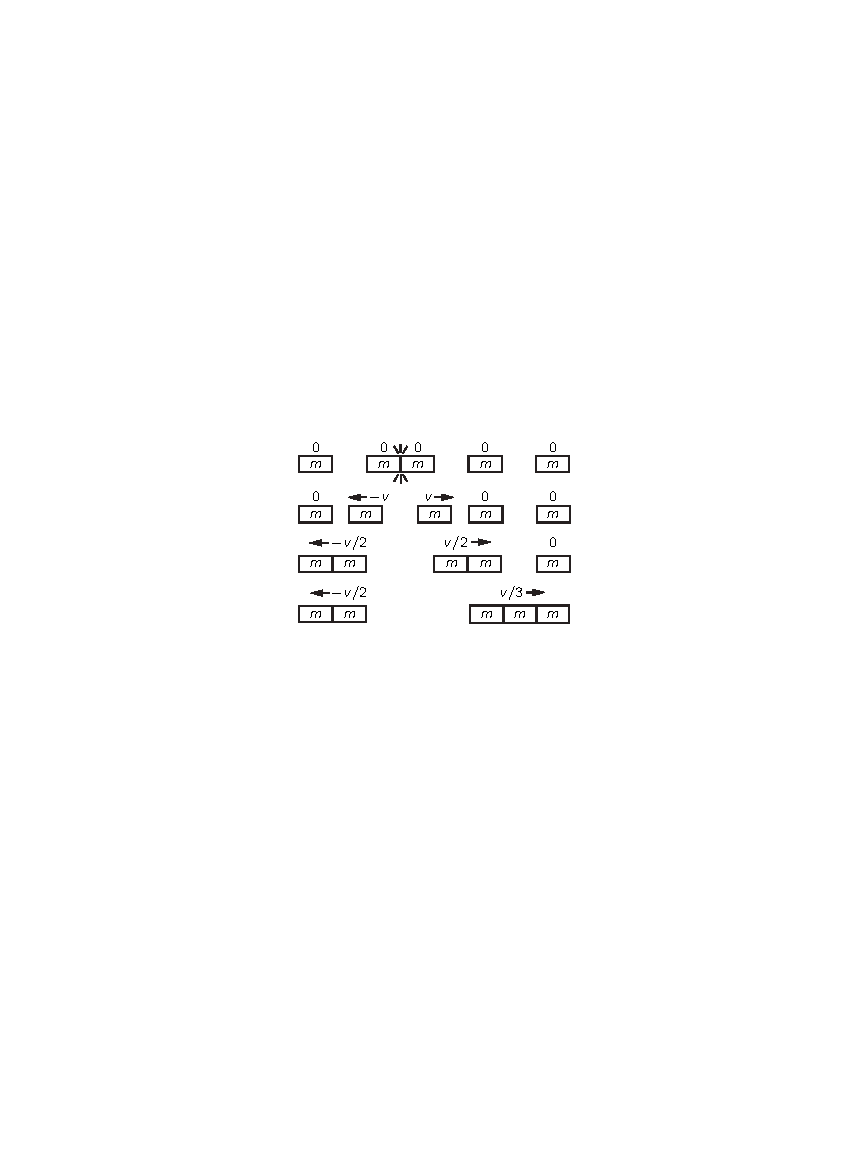
\includegraphics[width=5cm]{Chapter10/2m和3m之间的作用与反作用}    
        \caption{$2m$和$3m$之间的作用与反作用}
        \label{figure:2m和3m之间的作用与反作用}
    \end{minipage}
\end{figure}

现在的情况是1对2。利用同样的论证,我们可以预言1对3,2对3等等的结果,从静止开始的2对3的情况如图\ref{figure:2m和3m之间的作用与反作用}所示。

在每一种情况中,我们发现,第一个物体的质量乘它的速度,加上第二个物体的质量乘它的速度,等于最后物体的总质量乘它的速度。因此,这都是一些动量守恒的例证。从简单的、对称的情况出发,我们用实验说明了在较复杂情况下的守恒定律。事实上,对于任何质量比是有理数的情况,我们都能这样做,并且由于任何一个比值都可以充分接近于一个有理 数的比值,因此,我们能够以任何精确度处理任何比值的情形。

\section{动量和能量}

上述的所有例子都是物体发生碰撞结合在一起,或者是先结合在一起,以后又由于爆炸而被分开的简单的情况。然而也有一些物体不粘合在一起的情况;例如,两个质量相等的物体以相同速率发生碰撞后弹开。在很短的时间内,它们发生接触,彼此都受到压缩。在压缩最大的那一瞬间,它们的速度都是0,而能量则贮存在弹性物体内,就像压缩弹簧的情形一样。这个能量是由物体碰撞之前所具有的动能转化而来的,而在速度为0的那一瞬间,它们的动能就变为0。然而,动能只是暂时失去。压缩状况类似于爆炸时释放能量的雷管。在某种爆炸的状况下,这些物体立即膨胀并又相互飞开;但是我们已经知道在这种情况下,物体是以相同速率飞开的。然而,一般说来,弹开的速率要比原来的速率小,因为并非所有的能量都为爆炸所用,这与材料性质有关。如果材料是油灰,动能就不会恢复;如果材料是比较硬的,通常会再获得一定的动能。在碰撞中,其余的动能转化为热和振动能——物体变热并作振动。振动能量也很快转变为热能。用钢这样的高弹性材料制成一些碰撞物体,再用精心设计的弹簧缓冲器,有可能使得在碰撞中产生的热和振动很小。在这些情形中,弹回来的速度实际上等于初始速度;这种碰撞称为弹性碰撞。

弹性碰撞的前、后速度相等这件事与动量守恒无关,而与动能的守恒有关。然而,在对称的碰撞后,物体弹开的速率彼此相等却与动量守恒有关。

我们可以类似地分析不同质量、不同初始速度和不同弹性程度的物体之间的碰撞,确定最终速度和动能的损失,但是我们将不去详细探讨这些过程。

对于没有内部的“齿轮、转轴或部件”的系统来说,弹性碰撞是特别有趣的。这样在发生碰撞时,没有地方可以消耗能量,因为那些弹开的物体与它们在碰撞时的状态相同。因此,在非常基本的物体之间的碰撞总是高弹性的,或者非常接近于弹性的。例如,气体中分子或原子间的碰撞就被认为是完全弹性的。虽然这是一个非常好的近似,但即使这样的碰撞也不是完全弹性的;不然人们就会无法理解能量怎么会以光或热辐射的形式从气体中释放出来。在气体分子的碰撞中,偶尔会有低能红外线发射出来,但这种情况是非常罕见的,所发射的能量也是非常微小的。所以,对于大多数场合,气体中的分子碰撞被认为是完全弹性的。

作为一个有趣的例子,让我们考虑两个质量相等的物体之间的弹性碰撞。如果它们以同样速率相碰撞,那么,根据对称性原理,它们应当以相同的速率弹开。但是现在我们来看一下另一种情况下的这种碰撞,即其中的一个物体以速度$v$运动,而另一个物体保持静止。当两者碰撞时会出现什么情况?其实我们在前面已碰到过这种情况。从跟着物体中的一个一起运动的汽车中来观察对称的碰撞,我们发现,如果静止的物体与另一个质量恰好相同的物体发生弹性碰撞,则运动着的物体停了下来,而曾经是静止的物体现在以另一个物体曾经具有的同样的速度运动;两个物体只不过变换一下速度而已。用适当的碰撞装置很容易演示这个现象,更一般地说,假如两个物体以不同的速度运动,那么在碰撞时它们仅仅简单地交换一下速度。

另一个几乎是完全弹性的相互作用的例子为磁性。假如在我们的滑块上放置一对U形磁铁,使它们彼此推斥,那么当一块磁铁静静地移向另一块磁铁时,这块磁铁会把另一块推走,而自己则完全保持静止,被推走的一块磁铁则无摩擦地向前滑动。

动量守恒原理是非常有用的,因为它使我们在无需了解细节的情况下也能解决许多问题,例如,我们并不知道在雷管引爆时气体的运动情况,然而却能预知物体分离的速度。另一个有趣的例子是火箭的推进。一枚具有很大质量$M$的火箭用极大的速度$V$(相对于火箭来说)排出质量为$m$的小块后,如果火箭原来静止的话,它将以很小的速度$v$运动。利用动量守恒原理,我们可以计算出这个速度为
\begin{equation*}
    v=\frac{m}{M} \cdot V
\end{equation*}
只要不断地排出物质,火箭就一直加速。火箭的推进本质上与枪支的反冲是一回事:不需要任何作反推的空气。

\section{相对论性动量}

近代已对动量守恒定律作了一些修正。然而,今天这条定律仍是正确的,修正主要是在事物的定义上。在相对论中,我们的确也有动量守恒定律;粒子具有质量,而动量仍由$mv$,即质量乘以速度给出,但是质量随速度而改变,因此动量也发生改变。质量随速度的变化遵从以下规律
\begin{equation}
    \label{Eq:I:10:7}
    m=\frac{m_0}{\sqrt{1-v^2/c^2}}
\end{equation}
这里$m_0$。是物体的静止质量,$c$是光速。从这个公式很容易看出,除非$v$非常大,否则$m$与$m_0$的差别就可忽略,而对通常的速度,动量的表示式就还原为原来的公式。

单个粒子的动量分量可以写为
\begin{equation}
    \label{Eq:I:10:8}
    \begin{split}
        p_x=\frac{m_0v_x}{\sqrt{1-v^2/c^2}} \\
        p_y=\frac{m_0v_y}{\sqrt{1-v^2/c^2}} \\
        p_z=\frac{m_0v_z}{\sqrt{1-v^2/c^2}}
    \end{split}
\end{equation}
这里$v^2=v^2_x+v^2_y+v^2_z$。如果对所有相互作用粒子在碰撞前后的$x$动量分量分别求和,则两个和相等,也就是说,在$x$方向上的动量守恒。同样的情况对任何方向都成立。

在第4章中,我们看到,只有承认能量可表现为电能、机械能、辐射能、热能等等不同形式,能量守恒定律才确实成立。在某些这类情况中,例如热能,能量可以说成是“隐藏”的。这个例子可能使我们联想到这样一个问题:“是不是也存在着动量的隐藏形式——或许是某种热动量呢?”答案是由于下述理由隐藏动量是很困难的。

如果把各个原子的速度的平方相加,一个物体内原子的无规则运动就提供了热能的一种量度。速度平方和将是正的,不具有方向上的特征。物体内热的存在与物体是否作整体运动无关,并且以热这种形式的能量守恒不是很明显的。相反,如果我们把速度相加,由于速度是有方向的,若发现其结果不为零,这就意味着整个物体在某个特定方向上有移动,而这样显著的动量是很容易观察到的。因为只有物体作整体运动时,它才有净动量,所以就不存在内部无规则动量损耗。因此动量作为一个力学量是难以隐藏起来的。然而,例如在电磁场内动量也可以被隐藏起来。这种情况是另一种相对论效应。

牛顿的前提之一是认为在一段距离内的相互作用是瞬时的。结果发现情况并非如此;比如,在包含着电力的情况下,如果在某一个位置上的一个电荷突然移动,其对在另一个位置上的另一个电荷的影响并不是瞬时的——稍有一点延迟。在那种状况下,即使彼此作用的力是相等的,动量仍与之不符;这样,在一段短时间内将出现麻烦,因为有一段时间,第一个电荷将感受一定的反作用力,即获得了某些动量,但第二个电荷却丝毫也不受影响,也不改变它的动量。这段时间就是电作用跨过它们之间的距离所需要的时间,即以$186000~mi \cdot s^{-1}$的速度跨过这段距离的时间。在这段很短的时间内,粒子的动量是不守恒的。当然,在第二个电荷感受到第一个电荷的作用并且一切都稳定下来之后,动量的方程就完全成立,但在那段小小的时间间隔中动量是不守恒的。为了表明这一点,我们说在这段时间内除粒子的动量$mv$外还有另一类动量存在,这就是电磁场的动量。如果我们将电磁场的动量加在粒子的动量上,则在所有时间内动量每一时刻都守恒。电磁场具有动量和能量这个事实使场的存在更为真实。因此,更好的理解是,原来那种认为只有粒子之间存在力的概念必须修正为:粒子具有场,场作用在另一个粒子上,而场本身具有我们所熟悉的性质,比如正像粒子那样带有能量和动量。再举另外一个例子:电磁场中存在着我们称之为光的电磁波,结果光也具有动量。所以,光撞击一个物体时,它在每秒钟内传递了一定大小的动量;这相当于一个力,因为,如果被照射物体每秒钟获得一定的动量,它的动量就会发生变化,这种情况与有一个力作用在它上面完全相同。光撞击在物体上时会施加一个压力;这个压力很小,但用足够灵敏的仪器可以测量出来。

在量子力学中,动量是另一回事——它不再是$mv$了。物体的速度的含义已难以确切定义,但是动量仍然存在。在量子力学中,差别在于当粒子表现为粒子时,动量仍是$mv$,但是当粒子表现为波时,动量就用每厘米的波数来量度:波数越大,动量就越大。尽管存在这些差别,动量守恒定律在量子力学中仍然成立。虽然$f=ma$不成立,所有从牛顿定律出发的有关动量守恒的推导也都不成立,然而,在量子力学中,这条特殊定律却最后仍然保持有效!